	\subsection{Beispiel: $2p \rightarrow 1s$ Wasserstoff: Spontane Emission}
		\begin{figure*} [h]
			\begin{center}
				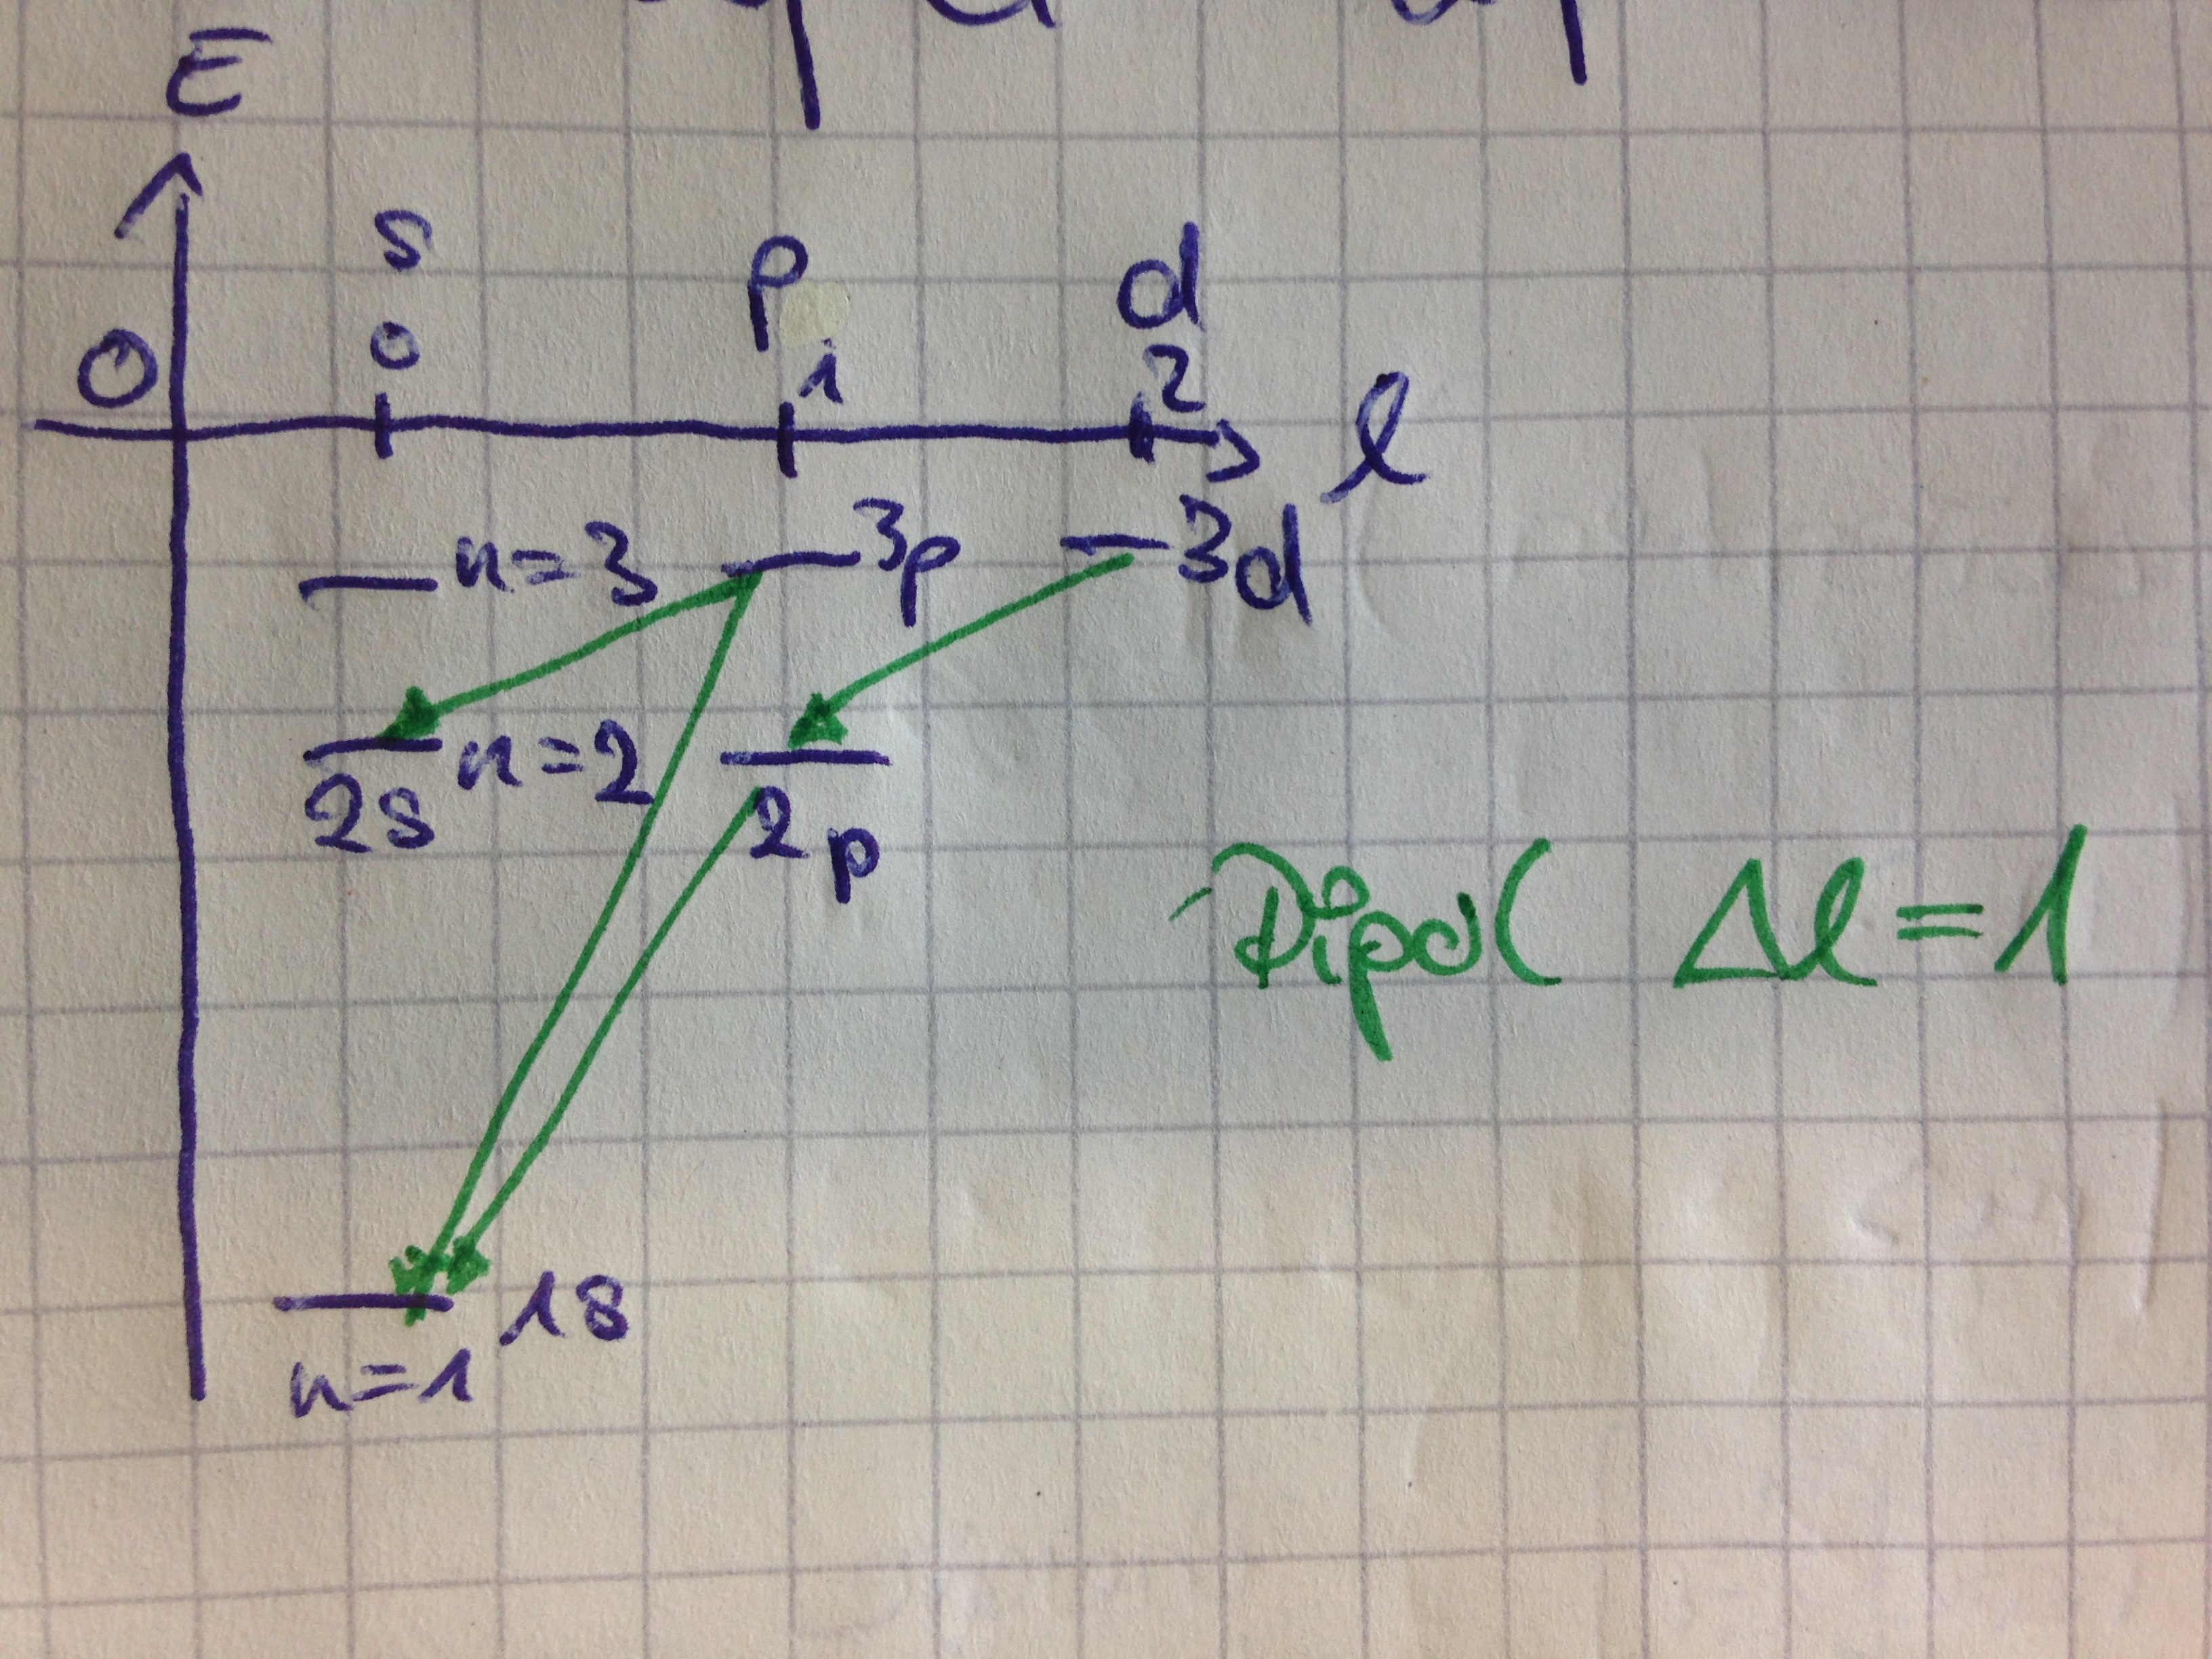
\includegraphics[width=10cm]{Bild3.jpg}
			\end{center}
		\end{figure*}
	Überrgangsrate:\marginpar{02.11.2015}
		\begin{align*}
			W_{f \leftarrow i} &=
			\frac{4}{3} \frac{\alpha ~\omega_{if}^3}{c^2} 
			\left|\braket{f | \vec{r} | i}\right|^2
			& &\left( \text{Einheit}: ~\frac{1}{\text{Zeit}}\right)
		\end{align*}
	Leistung
		\begin{align*}
			P &= \hbar \omega_{if} ~W_{f \leftarrow i} ~N_{H_{2p}} \propto \omega_{if}^4
		\end{align*}
	Hierbei ist $\hbar \omega_{if}$ die Energie und $N_{H_{2p}}$ die Anzahl der Wasserstoffatome im 2p Zustand.
		\begin{align*}
			\omega_{if} &= 
			\left( \frac{1}{n_f^2} - \frac{1}{n_i^2}\right)
			\frac{m c^2}{2 \hbar} \left(Z \alpha\right)^2
			= \frac{3}{8} \frac{m c^2}{\hbar} \left(Z \alpha\right)^2
		\end{align*}
	Hier: $n_f = 1, n_i = 2$ und die Summe in Klammern ist $>0$ da die Energie im Coulombpotential $<0$ ist.
		\begin{align*}
			\psi_{n \ell m} (\vec{r}) &= 
			\underbrace{\frac{u_{n \ell} (r)}{r}}_{\mathclap{R_{n \ell} (r)}}
			Y_{\ell m} (\Theta, \phi)
		\end{align*}
	Wir haben hier die Laguerre Polynome und somit:
		\begin{align*}
			u_{10} (r) &=
			2r \left(\frac{Z}{a_B}\right) e^{-\frac{Z r}{a_B}} \\
			u_{21} (r) &=
			\frac{2 r^2}{\sqrt{3}} \left(\frac{Z}{2 a_B}\right)^{\frac{3}{2}} e^{-\frac{Zr}{a_B}}
		\end{align*}
		\begin{align*}
			\frac{\vec{r}}{r} &=
			\sqrt{\frac{4\pi}{3}} 
			\left[
				\frac{1}{\sqrt{2}} \left(- Y_{11} + Y_{1-1}\right),
				\frac{1}{\sqrt{2}} i\left(Y_{11} + Y_{1-1}\right),
				Y_{10}
			\right]
		\end{align*}
	Winkelanteil von $\braket{i | \vec{r} | f}$ (Hier umgedreht, damit wir nicht komplex konjugieren müssen und wir den Braket sowieso ins Betragsquadrat nehmen.)
		\begin{align*}
			&\braket{\ell = 1, m | \vec{r} | 0~0} = & 
			&(\text{Auswahlregel~} \Delta \ell = 1) \\
			&= r \sqrt{\frac{4 \pi}{3}} \int \diff \Omega Y_{\ell m}^* (\Omega)
			\begin{pmatrix}
			\frac{1}{\sqrt{2}} \left(- Y_{11} + Y_{1-1}\right) \\
			\frac{1}{\sqrt{2}} i\left(Y_{11} + Y_{1-1}\right) \\
			Y_{10} \\
			\end{pmatrix}
			Y_{00}\\
			&= \frac{r}{\sqrt{6}} \delta_{\ell 1}
			\left( -\delta_{m1} + \delta_{m,-1}, i\delta_{m1} + i\delta_{m,-1}, \sqrt{2} \delta_{m0}
			\right)
		\end{align*}
	Radialintegral: 
		\begin{align*}
			\int_{0}^{\infty} \diff r ~r^2 \frac{u_{21} (r)}{r} ~r~ \frac{u_{10} (r)}{r} &=
			\int_{0}^{\infty} \diff r ~r~ u_{21} (r) ~ u_{10} (r) \\
			&= \frac{1}{\sqrt{6}} \left(\frac{Z}{a_B}\right)^4 
			\int_{0}^{\infty} \diff r ~r^4 e^{- \frac{3}{2} \frac{Zr}{a_B}} \\
			&= \left(\frac{2}{3}\right)^5 \frac{a_B}{Z} \frac{1}{\sqrt{6}}
			\underbrace{\frac{3}{2} \frac{Z}{a_B}
				\int_{0}^{\infty} \diff r \left(\frac{3}{2} \frac{Zr}{a_B}\right)^4
				e^{-\frac{3}{2} \frac{Zr}{a_B}}}_{\mathclap{4!}} \\
			&= \frac{a_B}{Z} \left(\frac{2}{3}\right)^5 \frac{24}{\sqrt{6}} 
			= \frac{a_B}{Z} \sqrt{6} ~\frac{2^7}{3^5}
		\end{align*}
	Jetzt benützen wir noch $(\delta_{m1})^2 = \delta_{m1}$ und $\delta_{m1}\delta_{m-1} = 0$ um den Erwartungswert auszurechnen:
		\begin{align*}
			|\braket{
				\overbrace{2~1~m }^{\mathclap{i}}| ~\vec{r}~ | \overbrace{1~0~0}^{\mathclap{f}}}|^2
				&= \frac{a_B^2}{Z^2} ~6~ \frac{2^{14}}{3^{10}} \frac{1}{6}
				\left(2 \delta_{m1} + 2 \delta_{m-1} + 2 \delta_{m0}\right) \\
				\Rightarrow W_{f \leftarrow i} &= 
				\frac{1}{3} \sum_{m=-1}^{1} \frac{4}{3} \frac{\alpha}{c^2}
				\left(\vphantom{\frac{3}{8}} \right.
					\underbrace{\frac{3}{8} \frac{m c^2}{\hbar} ~Z^2 \alpha^2}_{\mathclap{\omega_{if}}}
				\left. \vphantom{\frac{3}{8}} \right)^3 
				\frac{a_B^2}{Z^2} \frac{2^{15}}{3^{10}} 
				\left(\delta_{m1} + \delta_{m-1} + \delta_{m0}\right) \\
				&= \frac{2^8}{3^8} \frac{m c^2}{\hbar} Z^4 \alpha^5 
				\approx 6,3 \cdot 10^8 Z^4 s^{-1}
		\end{align*}
		